%% =====================================================================
%%  Extension of the submitted companion on correlated storage assignment
%%  in automated pick-and-pass warehouses. Venue-neutral working draft.
%%  Compiled by the authors on Overleaf; no journal class is used.
%%  The supplement (supplement.tex) is a separate document; the main text
%%  refers to its sections by name, so no cross-document package is needed.
%% =====================================================================
\documentclass[11pt]{article}

\usepackage{amsmath}
\usepackage{amssymb}
\usepackage{mathtools}
\usepackage{booktabs}
\usepackage{graphicx}
\usepackage{xcolor}
\usepackage{hyperref}
% APA references via BibTeX, as in the companion (without its journal class).
\usepackage[natbibapa]{apacite}

% Visible marker for every item that needs author confirmation or a verified source.
\newcommand{\authorreview}[1]{\textcolor{red}{[AUTHOR REVIEW: #1]}}

% Numbered propositions (kernel \newtheorem, no extra package).
\newtheorem{proposition}{Proposition}

% Working title (review round 1).
\title{Station workload shares after re-slotting a pick-and-pass warehouse: a held-out comparison of reserved margins and historical scenarios}
\author{\authorreview{author list and affiliations}}
\date{}

\begin{document}

\maketitle

% ---------------------------------------------------------------------
% Abstract, revised in review rounds 1 and 2 (at most 250 words).
% ---------------------------------------------------------------------
\begin{abstract}
In automated pick-and-pass warehouses, a layout that minimises station visits must also keep station workloads balanced on later orders. Where a companion study used per-station workload budgets, we state the limit as a two-sided rule on shares: each station's share of future workload must stay within a fixed absolute band around its historical share. Share-policy rows replace those budgets in the visit-minimisation model, under an information contract in which targets and scenarios come only from orders before a deployment origin. Two protections are compared: a margin reserved inside the band during optimisation, and robust rows over the product mixes of historical order blocks, extended to historically inactive products. After exploratory campaigns at an earlier origin of an industrial warehouse's order stream fixed the policy, a predeclared two-by-two comparison was deployed at a later origin and scored on orders not used by any earlier solve, score, or drift or dispersion analysis. Both configurations that reserved a margin satisfied the band on all three optimiser seeds, and neither configuration without one did on any seed; the configurations with historical scenarios kept the largest station deviation lower at higher mean visits per order. For every layout the later product mix lay outside the set of mixes it was protected against, and a sufficient condition on the distance between later and historical mixes did not hold. Reserving part of the band is thus a policy tested at one origin of one warehouse, not a calibrated rule.
\end{abstract}

\noindent\textit{Keywords:} storage location assignment; pick-and-pass warehouse; workload balancing; robust optimisation; constraint tightening; out-of-sample evaluation

% =====================================================================
\section{Introduction}\label{sec:introduction}
% =====================================================================
In an automated pick-and-pass warehouse a conveyor carries each order box past fixed picking stations, and the box diverts to every station that stores one of its products. The submitted companion paper \citep{belul_companion} poses correlated storage assignment for such systems with total order-station visits as the objective, under hard per-station limits on slots and workload, and applies it to an operating warehouse, Company~A. The workload limit exists because a layout that concentrates co-ordered products to save visits can route traffic to a few stations: a pick-and-pass line behaves as a network of queues \citep{yu2008pickandpass}, and a station whose arrival rate approaches its service rate blocks the main line \citep{kim2020}.

A layout is fitted to orders that have already been observed and is then operated on orders that come later. What the workload limit has to protect is therefore the distribution of work across stations on those later orders. The companion states the limit as a budget in workload units: each station's budget is 110\% of the complete legacy load it carried \citep{belul_companion}. Such a budget is tied to the volume of the horizon on which it was calibrated, whereas the volume of a future horizon is not known when the layout is chosen. This article studies a rule stated in shares instead: after re-slotting, each station should keep its share of future workload within a fixed number of percentage points of the share it carried historically under the layout the site operates. % AUTHOR-CONFIRM: whether Company A states its operational workload policy in these terms (AUTHOR_QUESTIONS.md, item 1).
A share rule needs no absolute workload level, since multiplying every product's workload by a common positive factor leaves every share unchanged. It does not make the horizon irrelevant, because a different horizon brings a different product mix.

The companion already evaluates its layouts out of sample: on a dated extract, a layout fitted to the first weeks and scored on the following weeks removes 6.6\% and 7.4\% of station visits, against 13.7\% in sample \citep{belul_companion}. Scoring layouts on later orders is thus already part of the companion's design. What the companion does not address is a share rule on later orders, and the choice between the ways of protecting such a rule that a planner can build into the optimisation. Three features of the problem shape that choice. First, the visit objective gives an optimiser no reason to leave part of a workload allowance unused, so a layout that satisfies a share rule on history may sit at the edge of the band at some station, where a small change in the product mix carries it outside. Second, the rule is two-sided: shares sum to one, so caps alone would let one station lose a large part of its work while the others absorb it, and a floor has to be protected as explicitly as a cap. Third, no static layout can keep a nontrivial band for every conceivable future, since a future whose work concentrates on the products of one station drives that station's share towards one; any protection therefore rests on an assumption about which futures matter.

Two standard responses are available. One reserves part of the band during optimisation and scores the layout at the full band, a device related to the protection levels of budgeted robust optimisation \citep{bertsimas2004price}. The other requires the band to hold for every product mix in a set built from historical variation, the set-inclusive form of robust optimisation \citep{soyster1973convex}. Here that set is the convex hull of the product mixes of historical order blocks, extended by activation protection, an allowance of workload mass on products that had no historical workload. The closest storage-assignment work states station balance on average demand and finds it exceeded under simulated demand variation \citep{winkelmann2025integrated}; Section~\ref{sec:related} positions the article against that work and the wider literature. Whether a reserved margin, historical scenarios, or both keep a visit-minimising layout inside a share band on later orders is an empirical question for a given site, and it is the question of this article.

We extend the companion's model to a share rule and compare the two responses on Company~A's order stream. The visit objective and the assignment structure are retained, and the per-station budget rows are replaced by rows that keep each station's share inside a two-sided absolute band around its historical target (Section~\ref{sec:model}). Workload counts product-order pairs rather than the companion's load normalised by processing rate, so the band is stated in shares of order lines, not in station utilisation. The rows are stated either over pooled history alone or over historical block scenarios with activation protection, and they are imposed either at the full band or at a band tightened by a reserved margin. An information contract fixes what is known when a layout is chosen: conditional on a snapshot of the catalogue and the incumbent layout, targets, training workloads and scenarios come from the orders before a deployment origin; the layout is frozen and then scored on the next $n$ complete orders (Section~\ref{sec:protocol}). Exploratory campaigns at an earlier origin shaped the rule and its parameters. A later origin then carried a predeclared two-by-two comparison of four model configurations, called arms, that crosses the reserved margin with scenario-and-activation protection; it was solved with three optimiser seeds and scored on orders that no earlier solve, score, or drift or dispersion analysis of the study had used.

% Contribution statement, revised in review round 1: held-out comparison first, formulation second, diagnostics third.
The article is a bounded comparative study, and its contribution has three parts. The first is held-out evidence on the two responses. Both arms that reserved a margin satisfied the band on all three optimiser seeds and neither arm without one did on any seed; in additional descriptive analyses, the arms with historical scenarios and activation kept their largest station deviations from target lower than the matching arms without them, at higher mean visits per order. The second is the share-policy formulation and information contract that make this comparison well posed: frozen targets, a closed catalogue in which frozen products keep their stations while their demand still counts, and a finite robust counterpart whose feasibility is conditional on the future product mix lying in the declared set. Its ingredients are standard (Section~\ref{subsec:rw_position}). The third is a set of diagnostics that bound the reading: the later product mix lay outside the set of mixes each returned layout was protected against, a sufficient condition on product-mix distance for the margin did not hold on any analysed window, and no validated rule for choosing the margin was obtained.

Section~\ref{sec:related} positions the study against the companion and the closest literature. Section~\ref{sec:model} states the information contract and the formulation. Section~\ref{sec:protocol} describes the data, the protocol, the staged design, the metrics and the scope of the evidence. Section~\ref{sec:results} reports the held-out comparison, then the exploratory context and additional descriptive analyses. Section~\ref{sec:discussion} discusses the findings and their limitations, and Section~\ref{sec:conclusion} concludes.

% =====================================================================
\section{Related work}\label{sec:related}
% =====================================================================
This section places the article among studies of workload balance in storage and station assignment, storage decisions under uncertain or changing demand, robust optimisation and out-of-sample evaluation, and it states what the article takes from each and where it differs from the closest work.

\subsection{Workload balance in pick-and-pass and zone storage}\label{subsec:rw_balance}
How work is spread over stations matters for the performance of a pick-and-pass line. \citet{yu2008pickandpass} approximate such systems as a queueing network to estimate order lead time and station utilisation, and use the approximation to evaluate storage methods at the stations. Balance has long been an aim of storage assignment itself. \citet{jane2000storage} assigns products to the zones of a relay picking line from historical orders so that pickers carry nearly equal loads, and adds heuristics that adjust locations when order volume fluctuates. \citet{tarczynski2023} formulates a mixed-integer model for pick-and-pass systems that minimises the maximum expected zone workload, and notes that assignment based on historical data carries risk, because even perfectly balanced zones can receive different workloads for a particular set of orders. \citet{kim2022dynamic} balance a weighted sum of picks and visits across the zones of a progressive bypass zone picking system and extend the model to reassignment under limited relocation capacity. \citet{zhang2024joint} impose a workload-balance constraint on picking aisles in a robotic mobile fulfilment system and report that robot movement distance increases as that constraint becomes more stringent. The companion \citep{belul_companion} minimises station visits subject to hard per-station budgets, each set at 110\% of the complete legacy load the station carried.

The closest work is \citet{winkelmann2025integrated}, who assign products to the stations and shelves of a pick-and-pass loop in an e-grocery fulfilment centre subject to constraints that bound each station's relative deviation in daily picks from the average over all stations from above and below. An assignment based on average demand exceeded a 3\% station deviation on individual days of the week against a 1\% threshold, and day-of-week-specific constraints brought the deviation below 1\%. Under simulated week-to-week variation with a coefficient of variation of 0.05, the maximum station deviation exceeded 4\% for the average-based assignment and still reached 2.46\% for the day-of-week-aware one. The authors suggest robust or stochastic optimisation for random variation as future work. Their study establishes that balance constraints set on average demand can be exceeded when demand varies. This article differs in four respects (Table~\ref{tab:closest}). Its targets are the frozen historical shares of each station under the incumbent layout, which differ from station to station, rather than the average over stations. Its band is absolute in share units rather than a relative deviation from that average. It protects the band against later demand with a reserved margin or with historical block scenarios rather than with day-of-week-specific constraints. It scores layouts on later observed orders of the same stream rather than on simulated weeks.

\begin{table}[htbp]
\centering
\caption{Closest studies to this article: how station or zone workload balance is stated, protected against demand change, and evaluated.}
\label{tab:closest}
\footnotesize
\setlength{\tabcolsep}{3pt}
\begin{tabular}{@{}p{2.2cm}p{2.3cm}p{2.7cm}p{2.6cm}p{2.5cm}@{}}
\toprule
Study & Setting & Balance rule & Protection against demand change & Evaluation \\
\midrule
\citet{tarczynski2023} & Pick-and-pass zones & Minimise the maximum expected zone workload & None; expected demand & Exemplary instances \\
\citet{kim2022dynamic} & Progressive bypass zone picking & Weighted picks and visits balanced across zones & Capacity-limited reassignment & Simulation with industry orders \\
\citet{winkelmann2025integrated} & Pick-and-pass loop & Upper and lower bounds on the relative deviation of daily picks from the average over all stations & Day-of-week-specific constraints & Simulated week-to-week variation \\
\citet{dundar2025robust} & Forward picking area & None & Budgeted robustness on correlation coefficients in the objective & Generated correlations, 5 to 12 SKUs \\
Companion \citep{belul_companion} & Pick-and-pass stations & One-sided budget, 110\% of legacy load & None & In sample; visits also on unseen dated weeks \\
This article & Pick-and-pass stations & Two-sided absolute band around each station's historical share & Reserved margin; historical block scenarios with activation & Later observed orders at one held-out origin \\
\bottomrule
\end{tabular}
\end{table}

\subsection{Storage decisions under uncertain or changing demand}\label{subsec:rw_uncertain}
Two lines of work respond to demand that is uncertain or changes over time. The first protects a plan. \citet{ang2012robust} model multiperiod storage and retrieval in a unit-load warehouse facing uncertain demand with partially characterised distributions, and minimise the worst-case expected total travel with a linear decision rule. \citet{dundar2025robust} derives a budgeted robust counterpart for correlated SKU-to-location assignment in which a budget limits how many uncertain correlation coefficients may deviate; the robustness applies to objective coefficients rather than constraints, no workload balance is modelled, and the author tests instances of 5, 10 and 12 SKUs and reports that larger instances become computationally intractable. Neither protects a workload restriction.

The second line changes the plan. \citet{christofides1973rearrangement} sequence the moves that rearrange a warehouse when relative demand changes, \citet{pazour2015reshuffling} optimise reshuffling by sequential moves, \citet{kim2022dynamic} limit reassignment to a relocation capacity, and \citet{wu2026reassignment} analyses when item storage should be reassigned as the demand pattern evolves in robotic mobile fulfilment. \citet{winkelmann2025integrated} observe that rearranging products is often not practical for short-term variation, whereas seasonal or long-term demand changes typically require it. The article takes no position on when to re-slot. It asks whether one re-slotting keeps the band on the orders that follow it.

Few of the reviewed studies score a storage allocation built from historical orders on orders that came later. \citet{mirzaei2021ica} build a cluster-based allocation from historical turnover and affinity and validate it on a real dataset in which 70\% of the orders, chosen at random, built the allocation and the rest were held out, a random rather than temporal split. \citet{waubertdepuiseau2022dslap} train a reinforcement-learning storage policy on one year of data and evaluate it on the following two months, a single temporal split. In the studies we reviewed, the companion and this article included, we found none that evaluates a storage decision across several successive origins.

\subsection{Robust optimisation ideas used here}\label{subsec:rw_robust}
The share rows of Section~\ref{sec:model} follow the set-inclusive, worst-case form of \citet{soyster1973convex}: a row must hold for every product mix in a declared set. \citet{bental1999robust} showed that robust counterparts of uncertain linear programmes can remain tractable, conic quadratic for ellipsoidal sets. Here the set is a polytope with finitely many relevant endpoints, so the counterpart consists of finitely many linear rows. \citet{bertsimas2003robust,bertsimas2004price} control conservatism with a per-constraint protection level that limits how many coefficients may deviate from their nominal values. The linear or integer structure is kept, and probabilistic bounds on constraint violation are attached. The reserve used in this article is different: a fixed fraction $\lambda$ of the band, subtracted on every share row, with no probabilistic bound attached. \citet{bertsimas2018datadriven} build uncertainty sets from data through statistical hypothesis tests, and their robust solutions carry finite-sample probabilistic guarantees. The scenario set used here is instead the convex hull of historical block mixes, extended by activation mass on historically inactive products; it is not a hypothesis-test set. Sampled-constraint methods relate feasibility to samples, through the exact feasibility of randomised solutions of uncertain convex programmes \citep{campi2008exact} or through sample approximations of chance constraints \citep{luedtke2008sample}.

The historical blocks of this article resemble sampled scenarios but do not meet the assumptions behind those guarantees. The guarantees of budgeted protection, of sample approximation and of distributionally robust data-driven decisions rest on independence or random-sampling assumptions \citep{bertsimas2004price,luedtke2008sample,vanparys2021data}. Consecutive blocks of one order stream are not randomly sampled, and their independence is not established. The model therefore claims only feasibility conditional on the future mix lying in the declared set, and the article implements none of the cited methods and tests none of their guarantees.

\subsection{Out-of-sample evaluation of optimised decisions}\label{subsec:rw_oos}
An optimised decision should not be judged on the data it was fitted to. \citet{smith2006optimizer} show that when alternatives are ranked by estimated value and the best is chosen, its true value should be expected to fall below its estimate even when the estimates are unbiased. \citet{vanparys2021data} define out-of-sample disappointment as the probability that the actual expected cost of a data-driven decision exceeds its predicted cost. The same reasoning, applied here to band compliance rather than cost, is why a layout optimised on history is scored on orders it was not fitted to. \citet{tashman2000outofsample} reviews out-of-sample tests of forecasting accuracy. \citet{cerqueira2020evaluating} note, following \citet{tashman2000outofsample}, that applying hold-out evaluation over multiple test periods gives more reliable estimates than a single partition, and their experiments on non-stationary series support this. By that standard the held-out evidence of this article is a single test period at one origin, preceded by an exploratory origin whose data it contains; the absence of further origins is a limitation of the study (Section~\ref{subsec:limitations}), not a gap it fills.

\subsection{What is standard and what this article adds}\label{subsec:rw_position}
Several components of the study are standard. Reserving part of a constraint is related to the protection levels of budgeted robust optimisation \citep{bertsimas2004price}, with the fixed-fraction difference stated in Section~\ref{subsec:rw_robust}. A linear row that holds at every point of a finite hull holds at its vertices, so worst-case rows over a scenario hull are a finite set of rows. Rescaling rows with integer data to integer counts with rounded thresholds uses only integrality. Scoring a decision on a later hold-out window is established in forecasting evaluation \citep{tashman2000outofsample,cerqueira2020evaluating}, and the companion already does so on unseen dated weeks, although few of the reviewed storage studies do (Section~\ref{subsec:rw_uncertain}). None of these is claimed as new.

Relative to the companion, the article replaces one-sided workload budgets by two-sided share rows under an explicit information contract. It compares a reserved margin with historical block scenarios in a predeclared factorial scored on later observed orders, and it reports diagnostics showing that the model's own feasibility does not explain the observed compliance. Relative to \citet{winkelmann2025integrated}, it differs in the respects stated in Section~\ref{subsec:rw_balance} and Table~\ref{tab:closest}, at the cost of evidence from one warehouse and one held-out origin. Among the studies reviewed, we found none that protects station workload-share constraints in pick-and-pass storage with a reserved margin or with scenarios built from historical orders and then scores the layouts on later observed orders; this is the article's reading of the reviewed set, not a claim about all published work.

% =====================================================================
\section{Information contract and share-policy formulation}\label{sec:model}
% =====================================================================
This section answers two questions: what a layout may use when it is chosen, and what its feasibility in the model promises for the orders that follow.

\subsection{What is known at a deployment origin}\label{subsec:contract}
The system is the companion's industrial system \citep{belul_companion}. $P$ is the catalogue of included products and $S$ the set of evaluated stations. Station $s$ has $\zeta_s$ storage locations, and $\sum_{s\in S}\zeta_s=|P|$. $P^{\mathrm{fix}}_s\subseteq P$ is the set of products frozen at station $s$, which keep that station in every layout. Every product occupies one slot whether or not its historical workload is zero, and it is movable unless it is frozen. The catalogue is closed: no product outside $P$ arrives in a later window. A layout is a binary matrix $x=(x_{ps})$, with $x_{ps}=1$ when product $p$ is stored at station $s$, that satisfies the assignment, slot-capacity and freeze rows \eqref{eq:assign}, \eqref{eq:cap} and \eqref{eq:fix} of Section~\ref{subsec:formulation}. Summing \eqref{eq:cap} over the stations bounds the number of placements by $\sum_{s}\zeta_s=|P|$, while \eqref{eq:assign} requires at least one placement per product, so each product is stored at exactly one station, every location is occupied, and a product can move only by exchange \citep{belul_companion}.

The unit of time is the complete order of the retained stream \authorreview{definition: state the loader's criterion for a complete order; no accepted source defines it}. Complete orders are indexed $0,1,2,\dots$ in the sequence of their order identifiers. A deployment origin $t$ splits this stream into the history $H_t$, the orders with index below $t$, and, for a horizon of $n$ complete orders, the future window $F_{t,n}$ of the orders with index from $t$ to $t+n-1$. For any window $W$, $O(W)$ is its set of orders, $P_o\subseteq P$ the set of products requested by order $o$, and $L_p(W)$ the number of orders in $W$ that request product $p$. Workload thus counts distinct product-order pairs, the counterpart of the companion's order lines $L_p$. It is not normalised by the processing rate $V_s$; neither $V_s$ nor the companion's budget $T_s$ is a parameter of the model below, and both appear only where row forms are compared. With $\Lambda(W)=\sum_{p\in P}L_p(W)>0$ the total workload of the window, the product mix of $W$ is the vector $\omega(W)$ on the simplex over $P$ with
\begin{equation}
\omega_p(W)=\frac{L_p(W)}{\Lambda(W)}\qquad\forall p\in P. \label{eq:mix}
\end{equation}
For a layout $x$, the share of station $s$ under a mix $\omega$ is
\begin{equation}
r_s(x;\omega)=\sum_{p\in P}x_{ps}\,\omega_p,\qquad \sum_{s\in S}r_s(x;\omega)=1, \label{eq:share}
\end{equation}
where the shares sum to one because each product is stored at exactly one station. Frozen products keep their stations, but their terms in \eqref{eq:share} change with $\omega$: freezing an assignment does not freeze its workload.

Let $x^0$ be the incumbent layout, the layout the site operates. The target of station $s$ is its historical share under that layout, computed once at the origin from the whole history and then frozen:
\begin{equation}
b_s=r_s\bigl(x^0;\omega(H_t)\bigr)\qquad\forall s\in S. \label{eq:target}
\end{equation}
Targets are never recomputed from the scored window or from the incumbent's profile on it. The information contract has two layers. Conditional on a snapshot of the catalogue, the incumbent layout, the slot counts, the freeze mask and the order-retention rule, all estimation (targets, training workloads and scenarios) uses only $H_t$, and each layout is written before its future window is scored. The snapshot itself is reconstructed from the whole export and assumed known before deployment, so the experiment is retrospective and snapshot-conditioned; prefix-only estimation under that snapshot is not evidence that the metadata were available at each historical origin. The order-retention rule is the loader's rule for which order lines, and hence which orders, are kept in the retained stream; it is reconstructed from the whole export and can depend on later orders \authorreview{definition: state the criteria of the order-retention rule, which the accepted sources do not give}. Section~\ref{subsec:data} describes the reconstruction.

\subsection{Retained structure and share-policy rows}\label{subsec:formulation}
The companion minimises total order-station visits subject to single-station assignment, slot capacity, linking rows and one-sided per-station workload budget rows \citep{belul_companion}. The extension keeps the objective and the assignment, capacity and linking rows, and it replaces the one-sided budget rows by two-sided share-policy rows. For a half-width $\delta\in(0,1)$ the two-sided absolute band of station $s$ is
\begin{equation}
\ell_s(\delta)=\max\{0,\ b_s-\delta\},\qquad u_s(\delta)=\min\{1,\ b_s+\delta\}. \label{eq:band}
\end{equation}
A layout satisfies the share policy on a window $W$ when $\ell_s(\delta)\le r_s(x;\omega(W))\le u_s(\delta)$ for every $s\in S$. The model is trained on the history with the training half-width
\begin{equation}
\bar\delta=(1-\lambda)\,\delta,\qquad 0\le\lambda<1, \label{eq:tight}
\end{equation}
so that $\lambda\delta$ is the margin reserved during optimisation. With $\lambda=0$ a layout is optimised at the full band; with $\lambda>0$ it is optimised inside a tightened band, and in both cases it is scored at $\delta$. For a modelled set $\mathcal U$ of product mixes (Section~\ref{subsec:uncertainty}) the training model reads
\begin{align}
\min\quad & \sum_{o\in O(H_t)}\sum_{s\in S} z_{os} \label{eq:obj}\\
\text{s.t.}\quad & \sum_{s\in S}x_{ps}\ge 1 && \forall p\in P, \label{eq:assign}\\
& \sum_{p\in P}x_{ps}\le\zeta_s && \forall s\in S, \label{eq:cap}\\
& x_{ps}\le z_{os} && \forall o\in O(H_t),\ p\in P_o,\ s\in S, \label{eq:link}\\
& x_{ps}=1 && \forall s\in S,\ p\in P^{\mathrm{fix}}_s, \label{eq:fix}\\
& \ell_s(\bar\delta)\le r_s(x;\omega)\le u_s(\bar\delta) && \forall s\in S,\ \omega\in\mathcal U, \label{eq:sharerow}\\
& x_{ps}\in\{0,1\},\quad z_{os}\in[0,1] && \forall o\in O(H_t),\ p\in P,\ s\in S. \label{eq:dom}
\end{align}
The objective \eqref{eq:obj} and rows \eqref{eq:assign} to \eqref{eq:link} and \eqref{eq:dom} are the companion's, written over the orders of the history; every such order counts, including orders that touch only frozen products. Row \eqref{eq:fix} states the frozen assignments, which the companion's industrial case expresses by handing the optimiser the residual slots of each station. The two-sided share-policy rows \eqref{eq:sharerow} replace the companion's one-sided budget rows; they are not added to them, and their floors have no counterpart in the companion's model. Share preservation is therefore a feasibility policy, and the objective remains the historical visit count. On the companion's set-variable representation, where $\Phi_s$ holds the products assigned to station $s$, the share is $r_s=\sum_{p\in\Phi_s}\omega_p$, and \eqref{eq:sharerow} restates on the partition $\{\Phi_s\}_{s\in S}$ as the companion's budget rows do.

The band is absolute: every station receives the same allowance in share units whatever its target, so at $\delta=0.02$ each station may move two percentage points on either side. A band relative to $b_s$ was not studied, and findings about the absolute band do not transfer to it. The half-width $\delta$ is also not the companion's tolerance of 10\% above a station's legacy load \citep{belul_companion}.

The share rows relate to budgets in one precise sense. The companion's budget row is $\sum_{p\in P}x_{ps}\,L_p/V_s\le T_s$ \citep{belul_companion}. Take a single scenario, $\mathcal U=\{\omega(W)\}$ for a fixed window $W$, with no activation. Multiplying the upper side of \eqref{eq:sharerow} by $\Lambda(W)$ gives $\sum_{p\in P}x_{ps}\,L_p(W)\le u_s(\bar\delta)\,\Lambda(W)$, which has the form of the companion's row with $V_s=1$ and $T_s=u_s(\bar\delta)\,\Lambda(W)$: a line-count budget proportional to the total workload of the window. Floors, rows over several scenarios and rows carrying activation terms are not budget rows. Multiplying every $L_p(W)$ by a common factor $c>0$ leaves every share, and so feasibility, unchanged, which is why the policy needs no absolute workload level. This is the only sense in which share rows stand in for budgets. Uniform scaling does not make the learned layout or its future compliance independent of the horizon: another $n$ changes the mix of the scored window and, through the historical blocks below, the modelled set.

\subsection{Modelled sets: pooled history, historical blocks and activation}\label{subsec:uncertainty}
The arms of the study differ in the modelled set $\mathcal U$ and in $\lambda$ (Table~\ref{tab:arms}). The smallest set is pooled history alone, $\mathcal U=\{\omega(H_t)\}$. Historical variation enters through blocks of the same length $n$ as the scored window. With $K_t=\lfloor t/n\rfloor$, block $B_k$ holds the orders with index from $t-kn$ to $t-(k-1)n-1$ for $k=1,\dots,K_t$, so the blocks are aligned at the origin, and
\begin{equation}
\Omega=\bigl\{\omega(B_1),\dots,\omega(B_{K_t}),\ \omega(H_t)\bigr\},\qquad \mathcal U^{\mathrm{H}}=\operatorname{conv}\Omega. \label{eq:hull}
\end{equation}
Products with no workload in the history, $P^0=\{p\in P:\ L_p(H_t)=0\}$, can still carry work later. When $P^0$ is nonempty, activation protection admits a workload mass of at most $\nu$ on them:
\begin{equation}
\mathcal U^{\mathrm{HA}}_\nu=\bigl\{(1-a)\,\omega+a\,v:\ \omega\in\operatorname{conv}\Omega,\ v\in\Delta(P^0),\ 0\le a\le\nu\bigr\}, \label{eq:activation}
\end{equation}
where $\Delta(P^0)$ is the set of mixes supported on $P^0$. When $P^0$ is empty, $\mathcal U^{\mathrm{HA}}_\nu$ is defined as $\operatorname{conv}\Omega$, and the model has no activation rows. The parameter $\nu$ is a mass budget shared by all of $P^0$, not a probability and not a budget per product. When $P^0$ is empty or $\nu=0$, $\mathcal U^{\mathrm{HA}}_\nu=\mathcal U^{\mathrm{H}}$ and the two corresponding arms are the same model.

The arm names follow this construction: NOM is the nominal model on pooled history, TIGHT the same model inside the tightened band, HIST the model over the historical block hull, and HIST+ACT the model over that hull with activation protection, while the suffix -T marks the tightened band.

\begin{table}[htbp]
\centering
\caption{Arms of the study. Each arm is the training model \eqref{eq:obj} to \eqref{eq:dom} with the modelled set and training half-width shown, and every arm is scored on its future window at the full half-width $\delta$.}
\label{tab:arms}
\small
\begin{tabular}{llll}
\toprule
Arm & Modelled set $\mathcal U$ & Training half-width & Held-out cell \\
\midrule
NOM & $\{\omega(H_t)\}$ & $\delta$ & (0,\,0) \\
TIGHT & $\{\omega(H_t)\}$ & $(1-\lambda)\delta$ & (0,\,1) \\
HIST & $\operatorname{conv}\Omega$ & $\delta$ & not run \\
HIST+ACT & $\mathcal U^{\mathrm{HA}}_\nu$ & $\delta$ & (1,\,0) \\
HIST+ACT-T & $\mathcal U^{\mathrm{HA}}_\nu$ & $(1-\lambda)\delta$ & (1,\,1) \\
\bottomrule
\end{tabular}
\par\smallskip
\begin{minipage}{0.92\linewidth}\footnotesize
Held-out cell: levels of (historical scenarios with activation, reserved margin) in the held-out factorial of Section~\ref{subsec:stages}. HIST ran only in the exploratory campaigns and HIST+ACT-T only in the held-out factorial.
\end{minipage}
\end{table}

For a fixed layout the share \eqref{eq:share} is linear in $\omega$ and in $v$ and affine in $a$. For nonempty $P^0$ its extremes over \eqref{eq:activation} are therefore attained at an element of $\Omega$, at an endpoint $a\in\{0,\nu\}$ and at a vertex $v=e_p$ with $p\in P^0$, where $e_p$ is the mix that places all workload on $p$. Write $\omega^k$ for the $k$-th element of $\Omega$ and $A_{sk}=r_s(x;\omega^k)$. For nonempty $P^0$, let $h_s(x)=\max_{p\in P^0}x_{ps}$, which is 1 when at least one product of $P^0$ is stored at $s$, and $g_s(x)=\min_{p\in P^0}x_{ps}$, which is 1 when every product of $P^0$ is stored at $s$. Then
\begin{align}
\max_{\omega\in\mathcal U^{\mathrm{HA}}_\nu}r_s(x;\omega) &= \max_{k}\ \max\bigl\{A_{sk},\ (1-\nu)A_{sk}+\nu\,h_s(x)\bigr\}, \label{eq:maxshare}\\
\min_{\omega\in\mathcal U^{\mathrm{HA}}_\nu}r_s(x;\omega) &= \min_{k}\ \min\bigl\{A_{sk},\ (1-\nu)A_{sk}+\nu\,g_s(x)\bigr\}, \label{eq:minshare}
\end{align}
because activation mass can raise the share of station $s$ only if some product of $P^0$ sits there, and can be kept away from $s$ only if some product of $P^0$ sits elsewhere. Over this set the rows \eqref{eq:sharerow} are therefore finitely many rows, linear in $x$ once $h_s$ and $g_s$ are represented; for the smaller sets the activation terms, or the blocks, drop out. In a linear model $h_s,g_s\in\{0,1\}$ are variables with $h_s\ge x_{ps}$ and $g_s\le x_{ps}$ for every $p\in P^0$. This is exact: $h_s$ enters only upper rows and $g_s$ only lower rows, each with a positive coefficient on the constrained side, so a layout satisfies the rows for some admissible $h_s$ and $g_s$ exactly when it satisfies them at $h_s(x)$ and $g_s(x)$. An earlier implementation omitted the term $\nu\,g_s$, which covers activation mass concentrated at one station; the correction changes no recorded result (Supplementary Section S3).

Multiplying each row by the integer workload total of its scenario, and the activation rows also by the denominator of $\nu$, gives rows with integer left-hand sides; replacing the thresholds by their floors in upper rows and their ceilings in lower rows defines the same set of layouts. The purpose is numerical: a solver whose feasibility tolerance is below one unit cannot accept a layout that violates an integer row. Exactness rests on the derivation in Supplementary Section S2. A solver return in finite precision is not an exact certificate, so every stored layout was revalidated in exact rational arithmetic by code that shares nothing with the solvers.

The first exploratory campaign (Section~\ref{subsec:stages}) used an upper-only rule, which keeps only the right-hand inequality of \eqref{eq:sharerow}. Because shares sum to one, caps alone imply only $r_s\ge\max\{0,\ 1-\sum_{j\ne s}u_j(\bar\delta)\}$, which on 24 stations in principle allows one station to lose far more than $\delta$ while the others absorb the work. Caps therefore bound a station's decrease of share only through that weak inequality, whereas floors bound it directly.

\subsection{Conditional feasibility, a sufficient margin condition and observed compliance}\label{subsec:conditional}
Feasibility in \eqref{eq:sharerow} is a statement about the futures in $\mathcal U$ and about nothing else.

\begin{proposition}
If a layout $x$ satisfies \eqref{eq:sharerow} for a modelled set $\mathcal U$ and the product mix $\omega(F_{t,n})$ of the future window lies in $\mathcal U$, then $\ell_s(\bar\delta)\le r_s(x;\omega(F_{t,n}))\le u_s(\bar\delta)$ holds for every $s\in S$ simultaneously, and so does the band with half-width $\delta\ge\bar\delta$.
\end{proposition}

The model provides conditional robust feasibility for its set under these assumptions. Nothing in it establishes that a future window lies in $\mathcal U$, and it assigns no probability to compliance; observed compliance on a scored window is one realisation. Membership can, however, be refuted station by station. If the realised share of some station lies above $\max_{\omega\in\mathcal U}r_s(x;\omega)$ or below $\min_{\omega\in\mathcal U}r_s(x;\omega)$, the future was outside $\mathcal U$; if every station lies within its range, membership is not proved. When $\mathcal U$ is the single point $\{\omega(H_t)\}$, the range of station $s$ is the single value $r_s(x;\omega(H_t))$, the layout's own share on history, and the station leaves it unless $r_s(x;\omega(F_{t,n}))=r_s(x;\omega(H_t))$. Membership is also a narrow condition. The hull $\operatorname{conv}\Omega$ of $K_t+1$ mixes has affine dimension at most $K_t$, whereas a mix has $|P|$ coordinates, and activation widens the set only in the directions of the inactive products; the set also contains fractional mixes that no window of $n$ orders produces.

A second, sufficient condition applies to arms that reserve a margin and whose set contains pooled history, that is TIGHT and HIST+ACT-T.

\begin{proposition}
For every layout $x$, station $s$ and mixes $\omega,\omega'$,
\begin{equation}
\bigl|r_s(x;\omega)-r_s(x;\omega')\bigr|\le\mathrm{TV}(\omega,\omega'):=\tfrac12\sum_{p\in P}|\omega_p-\omega'_p|. \label{eq:tv}
\end{equation}
Consequently, if $\ell_s\bigl((1-\lambda)\delta\bigr)\le r_s(x;\omega(H_t))\le u_s\bigl((1-\lambda)\delta\bigr)$ for every $s\in S$ and $\mathrm{TV}\bigl(\omega(F_{t,n}),\omega(H_t)\bigr)\le\lambda\delta$, then $x$ satisfies the band with half-width $\delta$ on $F_{t,n}$.
\end{proposition}

Because each product is stored at exactly one station, the share of $s$ is the mass that a mix places on the products stored at $s$, and two mixes differ on any set of products by at most their total-variation distance, which gives \eqref{eq:tv}. Hence $r_s(x;\omega(F_{t,n}))\le\min\{1,b_s+(1-\lambda)\delta\}+\lambda\delta\le b_s+\delta$, and since no share exceeds one, $r_s\le u_s(\delta)$; the floor follows in the same way. The condition is sufficient, not necessary, and the distance of a future window can only be measured after that window has been observed.

How much of its allowance a layout uses is measured by its minimum required slack on its own modelled set,
\begin{equation}
\eta(x;\mathcal U)=\max\Bigl\{0,\ \max_{s\in S}\max\bigl\{\max_{\omega\in\mathcal U}r_s(x;\omega)-b_s,\ \ b_s-\min_{\omega\in\mathcal U}r_s(x;\omega)\bigr\}\Bigr\}. \label{eq:slack}
\end{equation}
Because shares lie in $[0,1]$, the clipping in \eqref{eq:band} does not bind, and a layout satisfies \eqref{eq:sharerow} exactly when $\eta(x;\mathcal U)\le\bar\delta$. By \eqref{eq:target}, $\eta(x^0;\{\omega(H_t)\})=0$: the incumbent needs no slack on pooled history, whereas an optimised layout may spend its whole allowance. This asymmetry follows from defining the targets as the incumbent's own shares, and Section~\ref{sec:results} states it before the first comparison against the incumbent.

The parameters have distinct roles: $\delta$ is the policy half-width at which every layout is scored, $\lambda$ the fraction of it reserved during optimisation, and $\nu$ the activation mass of the modelled set. None of them is a numerical tolerance of the solver.

% =====================================================================
\section{Data, protocol and staged design}\label{sec:protocol}
% =====================================================================
This section specifies how the undated order stream is split into training and scoring windows, in which order the campaigns ran, and which metrics report them.

\subsection{Data and preprocessing}\label{subsec:data}
The data are the Company~A order export used by the companion, read through the companion's data loader without modification. The export records product, order, quantity, station and box fields and carries no dates. Horizons are therefore counted in complete orders taken in order-identifier sequence. That this sequence matches the creation, release, picking and delivery sequence on site is an assumption, which sorting does not establish. A dated protocol, such as the companion's unseen-week test, is a deferred alternative that this study does not disprove, and nothing here shows that dates are unnecessary for operational decisions in general. % AUTHOR-CONFIRM: whether order dates exist operationally at the site (AUTHOR_QUESTIONS.md, item 8).

The retained system has 284,862 complete orders, a catalogue of 21,874 products in 21,874 slots and 24 evaluated stations, with 5,899 products frozen and 15,975 movable. The companion reports 26 stations and evaluates the same 24, so no station is newly excluded here; the two other stations and their products enter neither the catalogue, the workloads, the visit counts nor any denominator. Stations are identified by the companion's aliases S1 to S24. Products are frozen by the companion's site rule \citep[Supplementary Section S6]{belul_companion}, whose order-frequency count the loader takes over large orders. That filter decides only which products form the movable decision pool: orders of every size remain in the evaluation stream, in the workloads and in the visit counts, and frozen products keep their stations while their changing demand still counts. On this export one product is an edge case, because duplicate entries in large orders leave it movable under the loader's count whereas a count of distinct orders would freeze it. The loader's classification, which preserves the companion's partition, is used, and workloads count distinct pairs throughout (Supplementary Section S4).

Industrial workload counts distinct retained product-order pairs, not units ordered or processing hours. Every included product occupies a slot even when its historical workload is zero, and no product outside the catalogue arrives in a later window; the catalogue is a closed snapshot, and an export cannot show that never-ordered physical inventory is complete.

\subsection{Order-indexed, horizon-conditioned protocol}\label{subsec:orderprotocol}
At a deployment origin $t$ the protocol computes the targets \eqref{eq:target}, the training workloads and the historical blocks from the orders before $t$ only, solves the training model of the arm, writes the returned layout, and only then scores it on the next $n$ complete orders $F_{t,n}$. Relative to the companion, whose unseen-week test splits a dated extract, this is an order-indexed evaluation with a later held-out deployment. The design has a single held-out period (Sections~\ref{subsec:rw_oos} and~\ref{subsec:scope}).

Horizons are counted in complete orders. At the exploratory origin the grid is $n\in\{\lceil|P|/2\rceil,\ |P|,\ 2|P|\}=\{10{,}937,\ 21{,}874,\ 43{,}748\}$, a declared sensitivity design rather than a recommended planning interval, and the historical blocks \eqref{eq:hull} of each run use the same $n$ as its scored window. At one origin, when the longer horizon is an integer multiple of the shorter, every block of the longer horizon is a union of blocks of the shorter one, so its modelled set is contained in the shorter horizon's set. This nesting constrains the model only. It implies nothing monotone about realised future compliance or about the visits of time-capped returned layouts, and it does not carry over to other horizons or origins. The held-out deployment uses $n=|P|$ only.

\subsection{Staged design}\label{subsec:stages}
The evidence comes from campaigns run in the order of Table~\ref{tab:design}. The order matters, because the policy of the held-out campaign was shaped by the exploratory ones.

The first campaign screened the arms NOM, TIGHT, HIST and HIST+ACT (Table~\ref{tab:arms}) under the upper-only rule with $\delta=0.01$, at the exploratory origin, order index 199,403, with one optimiser seed and the three horizons above, on a synthetic benchmark and on Company~A. After that campaign had been completed and reviewed, the rule was restated as two-sided, every station within $\pm\delta$ of its target. The primary half-width $\delta=0.02$ was chosen using the incumbent's largest station-share deviation in a single historical block on the exploratory prefix, and the reserved margin is $\lambda\delta$; no rule linking the margin to that statistic was tested (Section~\ref{subsec:descriptive}). A two-sided screen at $\delta=0.02$ on four synthetic warehouses and Company~A followed at the same origin, together with two sensitivity campaigns at $\delta=0.01$ and $\delta=0.03$ on Company~A. Their design was predeclared before their solves but after the same futures had been examined under the upper-only rule, so these campaigns are exploratory. \authorreview{value: solver, model representation and per-solve time limits of the exploratory campaigns, and the model representation of the held-out solves; not among the accepted values}

The held-out factorial was predeclared before any of its solves. It crosses two factors at two levels, historical scenarios with activation (absent or present) and the reserved margin (absent or present), which gives the arms NOM (0,\,0), TIGHT (0,\,1), HIST+ACT (1,\,0) and HIST+ACT-T (1,\,1). HIST was not run, because on Company~A it differs from HIST+ACT only by activation, which is not a factor of the design. The deployment origin is order index 243,151, the end of the furthest future scored at the exploratory origin, so the training history of the held-out deployment contains the exploratory origin's data and every future scored there. The policy was frozen before the held-out window was read: two-sided rule, $n=|P|=21{,}874$, $\delta=0.02$, $\nu=0.01$, $\lambda=0.5$, and optimiser seeds 11, 22 and 33. The 12 solves ran on Hexaly with one thread and a limit of 1,800~s each, 21,600~s configured in total. The scored window is the order index interval $[243{,}151,\ 265{,}025)$.

The retained stream holds 284,862 orders, so 19,837 retained orders follow the held-out window. They were used by no solve, score or analysis of this study, although the snapshot reconstruction of Section~\ref{subsec:data} read the whole export. That tail is shorter than $|P|$ orders but long enough for a smaller horizon; it was not read for this article, it is not designated for a further test, and it is not an independent warehouse.

\begin{table}[htbp]
\centering
\caption{Staged design of the study, in the order in which the campaigns were run.}
\label{tab:design}
\small
\begin{tabular}{@{}p{2.4cm}p{3.3cm}p{3.6cm}p{3.3cm}@{}}
\toprule
 & Upper-only screen & Two-sided screen and sensitivity & Held-out factorial \\
\midrule
Status & Exploratory & Exploratory; predeclared before its solves & Predeclared before any of its solves \\
Rule & Caps only & Two-sided band & Two-sided band \\
Half-width $\delta$ & 0.01 & 0.02 (screen); 0.01 and 0.03 (sensitivity) & 0.02 \\
$\nu$, $\lambda$ & 0.01, 0.5 & 0.01, 0.5 & 0.01, 0.5 \\
Origin (order index) & 199,403 & 199,403 & 243,151 \\
Horizons $n$ & 10,937; 21,874; 43,748 & 10,937; 21,874; 43,748 & 21,874 \\
Arms & NOM, TIGHT, HIST, HIST+ACT & NOM, TIGHT, HIST, HIST+ACT & NOM, TIGHT, HIST+ACT, HIST+ACT-T \\
Optimiser seeds & One & One & Three (11, 22, 33) \\
Data & Synthetic benchmark; Company~A & Four synthetic warehouses and Company~A (screen); Company~A (sensitivity) & Company~A \\
\bottomrule
\end{tabular}
\par\smallskip
\begin{minipage}{\linewidth}\footnotesize
Upper-only and two-sided results are reported separately and never pooled, and neither is pooled with the held-out factorial. Arms are defined in Table~\ref{tab:arms}; $\lambda$ applies to the tightened arms and $\nu$ to the arms with activation.
\end{minipage}
\end{table}

Across the analysed campaigns 412 cases returned a layout that was scored on its future window; because a layout shared by several cases is counted once, these cases hold 188 distinct layouts, and Supplementary Section S5 gives the full accounting.

\subsection{Metrics, endpoints and denominators}\label{subsec:metrics}
Every returned layout is scored on its future window with exact integer counts against rational thresholds, at zero tolerance. The metrics are the following.
\begin{itemize}
\item \textbf{Band compliance.} All 24 evaluated stations lie inside $[\ell_s(\delta),u_s(\delta)]$ on the window. Held-out counts are over three optimiser seeds; exploratory counts are over three horizons, read with the distinct layouts behind them.
\item \textbf{Breaches by direction.} The number of stations above the cap and below the floor, and the largest excess on each side in percentage points; the worst breach is the larger of the two.
\item \textbf{Largest deviation from target.} $\max_{s\in S}|r_s(x;\omega(F_{t,n}))-b_s|$ in percentage points, whether or not a station breaches.
\item \textbf{Visits.} Mean future station visits per order, that is the visits of the window's orders divided by $n$, and the saving in percent against the incumbent layout scored on the same window.
\item \textbf{Minimum required slack.} $\eta(x;\mathcal U)$ of \eqref{eq:slack} on the arm's own training set, as a share.
\item \textbf{Departures from the modelled set.} The number of stations, out of 24, whose realised share lies above $\max_{\omega\in\mathcal U}r_s$ or below $\min_{\omega\in\mathcal U}r_s$.
\end{itemize}

The predeclared primary endpoint required TIGHT to satisfy the band on the held-out window for at least two of the three optimiser seeds; failure would have closed the fixed-policy claim, and passing supports a bounded case-study claim only. The predeclared secondary reading is descriptive: for each arm, the seed-wise pass count, the breach magnitudes in both directions, the mean visits relative to the incumbent on the same window, and the departures from the modelled set in both directions. The comparison of largest deviations between arms, the visit ratio between arms, the minimum required slack, and the drift, dispersion and total-variation readings of Section~\ref{subsec:descriptive} were not predeclared and are reported as additional descriptive analyses. The incumbent is scored on the same window as context, not as a feasibility standard for the optimised arms. For each held-out solve the solver's relative gap and bound are recorded; both refer to the training visit objective \eqref{eq:obj}, not to future visits.

\subsection{Scope of the evidence}\label{subsec:scope}
The held-out evidence is one industrial warehouse, one deployment origin at order index 243,151, one horizon of $n=21{,}874$ complete orders and three optimiser seeds under one frozen policy with $\delta=0.02$, $\nu=0.01$ and $\lambda=0.5$. The seeds describe optimiser variability at that origin, not variation in future demand. They are averaged within the origin and never counted as separate futures, so no significance test or interval is computed, and nothing is claimed about other origins, horizons or warehouses. The study cannot separate historical scenarios from activation, which are bundled in the factorial, cannot isolate the reserved margin from solver and layout effects, and ran no $\lambda$, $\delta$ or $\nu$ frontier at the held-out origin. Every held-out layout is the best the solver returned within its time limit, so visit differences compare returned layouts, not optima. The exploratory campaigns have one seed at one origin, their three horizons share that origin, and they are reported separately from the held-out evidence.

% =====================================================================
\section{Results}\label{sec:results}
% =====================================================================
This section answers the question of Section~\ref{sec:introduction} first on the predeclared held-out comparison (Section~\ref{subsec:heldout}). It then reports the exploratory campaigns that shaped that comparison's policy (Section~\ref{subsec:exploratory}) and additional descriptive analyses of drift and historical variation (Section~\ref{subsec:descriptive}). The experimental unit and what the design cannot identify are stated in Section~\ref{subsec:scope}; held-out and exploratory results are never pooled.

% ---------------------------------------------------------------------
\subsection{The held-out factorial}\label{subsec:heldout}
% ---------------------------------------------------------------------
The held-out campaign asks whether a reserved margin, historical scenarios with activation, or both keep a visit-minimising layout inside the two-sided band on later orders. It deploys the four arms at order index 243,151 and scores each returned layout on the next 21,874 complete orders.

Every comparison with the incumbent layout below carries one asymmetry. The targets $b_s$ are the incumbent's own historical shares \eqref{eq:target}, so the incumbent starts with the whole allowance as headroom, whereas an optimised layout spends it. The incumbent's minimum required slack is 0 on the single history scenario on which NOM and TIGHT train, and about 0.0157 on the scenario set of HIST+ACT and HIST+ACT-T (the 11 historical blocks and the history scenario, with activation), which lies inside $\delta=0.02$ but above the tightened allowance of 0.01. The incumbent is scored on the same window as context, not as a feasibility standard for the optimised arms.

\paragraph{Primary endpoint.} TIGHT satisfied the two-sided band with $\delta=0.02$ on all three optimiser seeds, against a predeclared threshold of two, so the primary endpoint was met. The predeclaration names it the ``Replication endpoint''; it tests the same policy at a later origin of the same order stream, whose history contains the exploratory origin's data. Meeting it supports a bounded case-study claim about this policy at this origin.

\paragraph{Pass pattern and breaches.} The arms that satisfied the band are exactly the arms that reserved a margin: TIGHT and HIST+ACT-T satisfied it on 3/3 seeds, and NOM and HIST+ACT on 0/3 (Table~\ref{tab:heldout_seeds}). This is a two-factor comparison under equal configured solve budgets at one origin; it is not a causal law, and it does not isolate the margin from solver and layout effects. The misses of the two arms without a margin differ in size: the worst breach of HIST+ACT was at most 0.179 percentage points, and that of NOM, the unprotected (0,\,0) control, at least 0.939. NOM missed on both sides of the band on every seed; HIST+ACT missed below the floor on every seed and above the cap on two, and the table gives the counts and magnitudes on each side. A small breach is still a miss of the declared policy. The misses of NOM are reported here as the contrast given by the unprotected control, and those of HIST+ACT are discussed as a limitation in Section~\ref{subsec:limitations}. Figure~\ref{fig:heldout_visits_breach} places the 12 returned layouts by worst breach and visits, and Figure~\ref{fig:heldout_station_shares} shows at which stations each breach occurred.

\begin{table}[htbp]
\centering
\caption{Held-out outcome of each returned layout: origin 243,151, $n=21{,}874$, two-sided band with $\delta=0.02$ over the 24 evaluated stations.}
\label{tab:heldout_seeds}
\small
\setlength{\tabcolsep}{4pt}
\begin{tabular}{@{}llcrrrrrr@{}}
\toprule
 & & & \multicolumn{2}{c}{Above cap} & \multicolumn{2}{c}{Below floor} & Largest & Visits \\
\cmidrule(lr){4-5}\cmidrule(lr){6-7}
Arm & Seed & Band & Stations & Worst & Stations & Worst & deviation & per order \\
\midrule
NOM        & 11 & miss & 4 & 1.006 & 5 & 0.178 & 3.006 & 3.266 \\
           & 22 & miss & 4 & 0.939 & 4 & 0.233 & 2.939 & 3.256 \\
           & 33 & miss & 2 & 1.144 & 4 & 0.167 & 3.144 & 3.172 \\
\addlinespace
TIGHT      & 11 & pass & 0 & 0.000 & 0 & 0.000 & 1.756 & 3.266 \\
           & 22 & pass & 0 & 0.000 & 0 & 0.000 & 1.209 & 3.267 \\
           & 33 & pass & 0 & 0.000 & 0 & 0.000 & 1.357 & 3.276 \\
\addlinespace
HIST+ACT   & 11 & miss & 1 & 0.081 & 1 & 0.039 & 2.081 & 3.278 \\
           & 22 & miss & 2 & 0.085 & 2 & 0.179 & 2.179 & 3.239 \\
           & 33 & miss & 0 & 0.000 & 2 & 0.069 & 2.069 & 3.274 \\
\addlinespace
HIST+ACT-T & 11 & pass & 0 & 0.000 & 0 & 0.000 & 1.026 & 3.351 \\
           & 22 & pass & 0 & 0.000 & 0 & 0.000 & 1.160 & 3.386 \\
           & 33 & pass & 0 & 0.000 & 0 & 0.000 & 1.039 & 3.304 \\
\midrule
Incumbent  &    & pass & 0 & 0.000 & 0 & 0.000 & 1.157 & 3.847 \\
\bottomrule
\end{tabular}
\par\smallskip
\begin{minipage}{\linewidth}\footnotesize
Band: pass when every station's realised share lies in $[\max(0,b_s-\delta),\min(1,b_s+\delta)]$. Stations: number of stations beyond that side of the band. Worst: largest excess beyond it, in percentage points. Largest deviation: largest $|r_s-b_s|$ over the 24 stations, in percentage points. Visits per order: mean future station visits over the window's orders. Arms are defined in Table~\ref{tab:arms}; every optimised layout is time-capped. Incumbent: the site's layout, whose own historical shares define $b_s$, scored on the same window as context.
\end{minipage}
\end{table}

\begin{figure}[htbp]
\centering
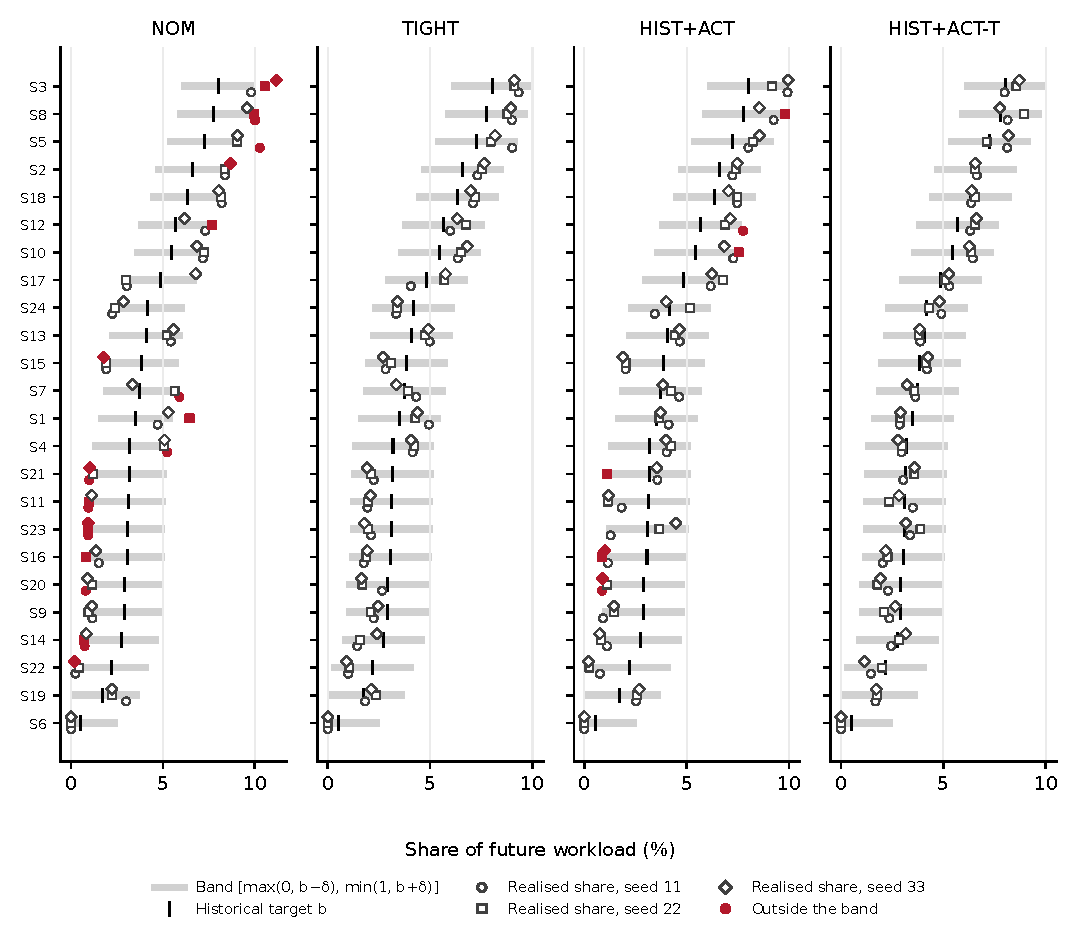
\includegraphics[width=\textwidth]{figures/fig_heldout_station_shares.pdf}
\caption{Realised future workload shares of the 24 evaluated stations on the held-out window (origin 243,151, $n=21{,}874$), one panel per arm. Rows are stations, labelled with the companion's aliases and sorted by historical target $b_s$ (black tick), which is computed on the orders before the origin under the incumbent layout and frozen. The grey bar is the band $[\max(0,b_s-\delta),\min(1,b_s+\delta)]$ with $\delta=0.02$. Markers give the realised share for each optimiser seed and are filled when the share lies outside the band. Shares are in percent.}
\label{fig:heldout_station_shares}
\end{figure}

\paragraph{Deviation from target and visits.} At both margin levels the arm with historical scenarios and activation kept the largest station deviation from target lower than the matching arm without them on every seed, and it had higher mean visits per order (Table~\ref{tab:heldout_arms}). With the margin, HIST+ACT-T kept its largest station deviation between 1.026 and 1.160 percentage points over the seeds, against 1.209 to 1.756 for TIGHT, and made 2.4\% more mean future visits per order than TIGHT; the visit ranges of these two arms do not overlap, whereas those of the two arms without the margin do. The scenario-and-activation arms thus kept the largest station deviation lower at higher mean visits per order; they did not change which arms satisfied the band. Scenarios and activation are bundled in this design, so their separate contributions are not identified, and the deviation comparison and the visit ratio are additional descriptive analyses of time-capped returned layouts. On the maximum-deviation statistic HIST+ACT-T, at most 1.160 over the seeds, is close to the incumbent's 1.157 on the same window; the statistic does not show that their station profiles are the same.

\begin{table}[htbp]
\centering
\caption{Held-out results by arm over three optimiser seeds, with the incumbent layout scored on the same window.}
\label{tab:heldout_arms}
\small
\setlength{\tabcolsep}{4pt}
\begin{tabular}{@{}lcccrc@{}}
\toprule
 & Seeds & \multicolumn{2}{c}{Visits per order} & Saving vs & Largest deviation \\
\cmidrule(lr){3-4}
Arm (scenarios, margin) & in band & Mean & [min, max] & incumbent (\%) & [min, max] (pp) \\
\midrule
NOM (0,\,0)        & 0/3 & 3.232 & [3.172, 3.266] & 16.0 & [2.939, 3.144] \\
TIGHT (0,\,1)      & 3/3 & 3.270 & [3.266, 3.276] & 15.0 & [1.209, 1.756] \\
HIST+ACT (1,\,0)   & 0/3 & 3.264 & [3.239, 3.278] & 15.2 & [2.069, 2.179] \\
HIST+ACT-T (1,\,1) & 3/3 & 3.347 & [3.304, 3.386] & 13.0 & [1.026, 1.160] \\
\midrule
Incumbent          & in band & 3.847 &  & (reference) & 1.157 \\
\bottomrule
\end{tabular}
\par\smallskip
\begin{minipage}{\linewidth}\footnotesize
Mean: arithmetic mean over the three seeds. [min, max]: range over the seeds. Saving: reduction of the arm's mean visits per order against the incumbent's 3.847 on the same window. The incumbent's targets are its own historical shares, so it starts with the whole allowance as headroom. Visits compare time-capped returned layouts, not optima.
\end{minipage}
\end{table}

\paragraph{Visits against the incumbent.} Every optimised arm made fewer visits per order than the incumbent, which made 3.847 on the same window: the arm-level means were 13.0\% to 16.0\% lower, and Table~\ref{tab:heldout_arms} gives each arm's saving next to its pass count. Single runs made 12.0\% to 15.1\% fewer visits for the two margin arms and 14.8\% to 17.5\% fewer for the two arms without a margin, all of them time-capped returned layouts. These savings are not comparable with the companion's figures \citep{belul_companion}. Its 13.7\% is measured in sample over the whole planning horizon rather than on a later window, and under station budget rows rather than a share band. Its 6.6\% and 7.4\% on unseen weeks come from a different dated extract, order stream, reference layout and workload restriction.

\begin{figure}[htbp]
\centering
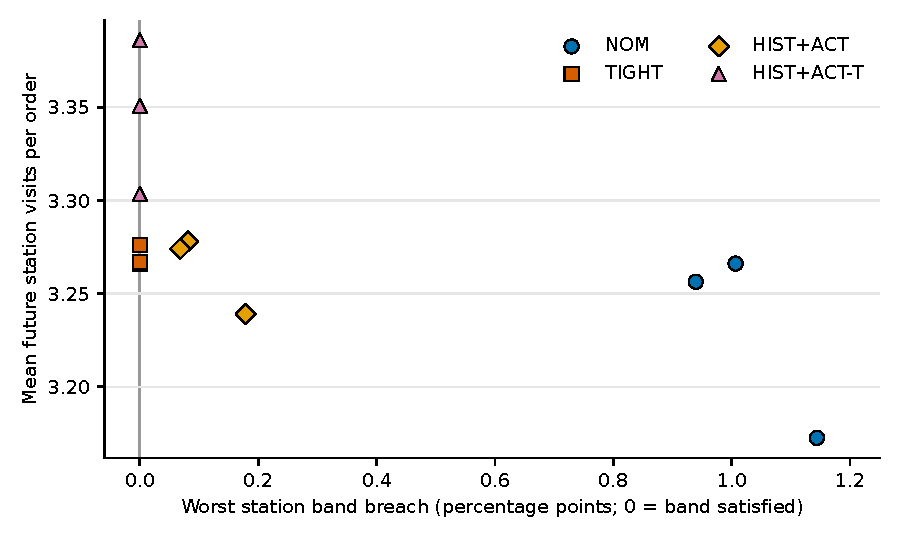
\includegraphics[width=0.85\linewidth]{figures/fig_heldout_visits_breach.pdf}
\caption{Held-out outcomes of the 12 returned layouts (four arms, three optimiser seeds each) at origin 243,151 with $n=21{,}874$: mean future station visits per order against the worst station band breach in percentage points, where 0 means that all 24 evaluated stations satisfied the two-sided band with $\delta=0.02$. Two TIGHT markers nearly coincide. The incumbent layout, which satisfied the band on the same window, made 3.847 visits per order and lies outside the plotted range. Every layout is time-capped, so visit differences compare returned layouts, not optima.}
\label{fig:heldout_visits_breach}
\end{figure}

\paragraph{Training allowance and the modelled set.} Every returned layout used almost exactly the training allowance its arm was given (Table~\ref{tab:heldout_diag}). The layouts without a margin required between 0.019997 and 0.019999 of the allowed 0.02, and the layouts with the margin between 0.009992 and 0.009999 of the allowed $(1-\lambda)\delta=0.01$. These values are measured on each arm's own training set, not on the future window, and they describe time-capped returned layouts; they are additional descriptive analyses.

The realised future lay outside the modelled set of every returned layout, mostly in the downward direction for the scenario arms (Table~\ref{tab:heldout_diag}). For NOM and TIGHT the modelled set is the single pooled-history point, which a station leaves unless its share is unchanged; all 24 stations lay off it on every seed, and those counts are not comparable with the scenario arms' counts. Leaving the modelled set is not a band violation: both margin arms left their sets and still satisfied the band. A departure at one station proves that the future was outside the set, whereas staying inside every station's range would not have proved membership.

\begin{table}[htbp]
\centering
\caption{Training-side diagnostics of the held-out layouts: minimum required slack \eqref{eq:slack} on each arm's own modelled set, and stations whose realised future share lay above or below the range of that set.}
\label{tab:heldout_diag}
\small
\setlength{\tabcolsep}{4pt}
\begin{tabular}{@{}lccccccc@{}}
\toprule
 & Training & \multicolumn{3}{c}{Minimum required slack (share)} & \multicolumn{3}{c}{Stations above / below the set} \\
\cmidrule(lr){3-5}\cmidrule(lr){6-8}
Arm & half-width & Seed 11 & Seed 22 & Seed 33 & Seed 11 & Seed 22 & Seed 33 \\
\midrule
NOM        & 0.02 & 0.019998 & 0.019999 & 0.019999 & 11 / 13 & 11 / 13 & 11 / 13 \\
TIGHT      & 0.01 & 0.009992 & 0.009996 & 0.009999 & 12 / 12 & 11 / 13 & 11 / 13 \\
HIST+ACT   & 0.02 & 0.019997 & 0.019997 & 0.019999 & 1 / 3 & 3 / 4 & 0 / 4 \\
HIST+ACT-T & 0.01 & 0.009993 & 0.009998 & 0.009998 & 0 / 2 & 1 / 4 & 0 / 4 \\
\bottomrule
\end{tabular}
\par\smallskip
\begin{minipage}{\linewidth}\footnotesize
Training half-width: $\delta=0.02$ without a margin and $(1-\lambda)\delta=0.01$ with it. The incumbent's minimum required slack is 0 on the history scenario of NOM and TIGHT and about 0.0157 on the scenario set of HIST+ACT and HIST+ACT-T. For NOM and TIGHT the modelled set is one point, which a station leaves unless its share is unchanged; all 24 lay off it, and their counts are not comparable with those of the scenario arms. Minimum slack is an additional descriptive analysis; departures are a predeclared secondary metric.
\end{minipage}
\end{table}

\paragraph{Solver returns.} All 12 held-out solves returned time-capped layouts with no proof of optimality. Each ended with a relative gap of about 98.5\% against a bound of 11,517 on the training visit objective \eqref{eq:obj}, not on future visits, so the bound gives no evidence that any returned layout is near optimal, and visit differences between arms compare returned layouts under equal configured budgets, not optimal values (Supplementary Section S1).

% ---------------------------------------------------------------------
\subsection{Exploratory context at origin 199,403}\label{subsec:exploratory}
% ---------------------------------------------------------------------
The campaigns in this subsection preceded the held-out factorial and shaped its policy. Each has one optimiser seed at one origin, and its three horizons share that origin, so they are not repeated draws. The two-sided policy was fixed before its solves but after the same futures had been examined under the upper-only rule.

\begin{table}[htbp]
\centering
\caption{Exploratory campaigns on Company~A at origin 199,403 with one optimiser seed: number of the three horizons $n\in\{10{,}937,\ 21{,}874,\ 43{,}748\}$ at which each arm satisfied the rule.}
\label{tab:exploratory}
\small
\begin{tabular}{@{}lccccc@{}}
\toprule
 & Layouts & Upper-only & \multicolumn{3}{c}{Two-sided} \\
\cmidrule(lr){4-6}
Arm & per campaign & $\delta=0.01$ & $\delta=0.01$ & $\delta=0.02$ & $\delta=0.03$ \\
\midrule
NOM      & 1 & 0/3 & 0/3 & 0/3 & 0/3 \\
TIGHT    & 1 & 0/3 & 1/3 & 3/3 & 3/3 \\
HIST     & 3 & 0/3 & 0/3 & 0/3 & 0/3 \\
HIST+ACT & 3 & 2/3 & 0/3 & 1/3 & 0/3 \\
\bottomrule
\end{tabular}
\par\smallskip
\begin{minipage}{\linewidth}\footnotesize
Layouts per campaign: distinct layouts behind the three horizons. NOM and TIGHT train on pooled history, which does not depend on $n$, so one layout is scored three times; HIST and HIST+ACT solve once per horizon, and counts of arms with different layout numbers are therefore not like counts. TIGHT uses $\lambda=0.5$ and the activation arm $\nu=0.01$. Exploratory evidence, never pooled with the held-out results.
\end{minipage}
\end{table}

\paragraph{Upper-only and two-sided rules.} The two rules order TIGHT and HIST+ACT differently (Table~\ref{tab:exploratory}). Under the upper-only rule with $\delta=0.01$, HIST+ACT satisfied the caps at two of the three horizons and NOM, TIGHT and HIST at none. Under the two-sided rule with $\delta=0.02$, TIGHT satisfied the band at all three horizons, HIST+ACT at one, and NOM and HIST at none. These are not like counts: each of NOM and TIGHT contributed one layout scored at three nested horizons, whereas HIST and HIST+ACT contributed three layouts. The different ordering is consistent with the size and side of the margin that each rule reserved for TIGHT. Its layouts required a training allowance of about 0.005 under the upper-only rule, so half a percentage point was reserved, on the cap side only; under the two-sided rule with $\delta=0.02$ they required about 0.010, so one percentage point was reserved on each side. Consistency with the margin size is not a causal isolation, and an upper-only pass limits increases only, so it does not show that station profiles were preserved (Section~\ref{subsec:uncertainty}).

Under the two-sided rule the misses of the scenario arms were mostly, but not only, below the floor: summed over the three horizons, HIST+ACT had 0 cap and 3 floor breaches and HIST 1 cap and 8 floor breaches. In every two-sided cell on Company~A the realised future also fell below the lowest modelled share at some station; leaving the modelled set and breaching the band are different metrics.

\paragraph{Band width.} Each value of $\delta$ is a separately optimised model and a separate solve. With $\delta=0.03$, TIGHT satisfied the band at all three horizons and NOM, HIST and HIST+ACT at none; with $\delta=0.01$, TIGHT satisfied it at one horizon and the other arms at none, with the same layout counts as above. A wider band did not bring the scenario arms into compliance at this origin, and the narrower band was met once. The three values of $\delta$ form a sampled response, not a frontier. No lower bound was certified, so no band is shown to be out of reach, and no $\lambda$ frontier was run.

\paragraph{Synthetic instances.} Synthetic instances enter the exploratory campaigns as a control on finite-sample and solver effects, not as evidence about robustness to drift, because their generator is stationary. Under the two-sided rule they consist of 4 warehouses at one origin with one seed. Their sets of historically inactive products are empty, so HIST+ACT is the same model as HIST on them; that equality is an identity, not evidence that activation protection is costless or beneficial. Under the upper-only rule the larger synthetic screen supports no single ranking of historical scenarios against tightening: the comparison is mixed across catalogue-size strata and rests on unequal scored denominators, because the scenario arms returned no layout within the time limit in part of the smallest family, which is not infeasibility. Supplementary Section S5 reports the synthetic outcomes, including the cells without a returned layout.

% ---------------------------------------------------------------------
\subsection{Additional descriptive analyses: drift, a sufficient margin condition and historical variation}\label{subsec:descriptive}
% ---------------------------------------------------------------------
The analyses in this subsection were not predeclared endpoints. They describe how far the scored windows moved from history and how the reserved margin compares with the site's historical station-level variation. The drift analysis was computed after the held-out window had been scored; the margin was not chosen from it and is not re-chosen after the result.

\begin{table}[htbp]
\centering
\caption{Additional descriptive analyses: total-variation distances of product mixes and the incumbent's historical station-share deviations, against two references.}
\label{tab:context}
\small
\begin{tabular}{@{}p{6.4cm}cc@{}}
\toprule
Quantity & Stored & Like for like \\
\midrule
\multicolumn{3}{@{}p{10.4cm}}{\emph{Total-variation distance from pooled history; history before order index 243,151, blocks of $n=21{,}874$ orders}} \\
Largest of the 11 historical blocks & 0.194 & about 0.214 \\
Held-out window, ex post & 0.195 & not applicable \\
\midrule
\multicolumn{3}{@{}p{10.4cm}}{\emph{Incumbent's largest station-share deviation in one historical block (pp); history before order index 199,403}} \\
$n=10{,}937$ & 1.70 & about 1.80 \\
$n=21{,}874$ & 1.63 & about 1.83 \\
$n=43{,}748$ & 1.47 & about 1.89 \\
\bottomrule
\end{tabular}
\par\smallskip
\begin{minipage}{\linewidth}\footnotesize
Stored: each block measured against a pooled history that contains it. Like for like: against the rest of the history, obtained by dividing the stored value by one minus the block's mass fraction; block line mass is not stored, so the fraction is taken by order count (about 0.09 for the held-out history). The stored mean over the 11 blocks is 0.171. The deviations belong to the incumbent layout and exist only for the exploratory history. None of these values was a predeclared endpoint.
\end{minipage}
\end{table}

\paragraph{Product-mix drift.} Measured against the rest of the history, the largest historical block distance is about 0.214, and the held-out product mix, at a total-variation distance of 0.195 from the pooled history against which it was scored, lies below it (Table~\ref{tab:context}). The stored historical maximum of 0.194 measures each block against a pooled history that contains that block, which shrinks each value by the factor one minus the block's mass fraction (Supplementary Section S6). Block line mass is not stored, so that fraction is taken by order count, about 0.09; the stored ordering reverses for any mass fraction above about 0.0028. The incumbent layout satisfied the two-sided band on the held-out window. Total-variation distance measures change in the product mix, not change in station shares, because changes among the products of one station can cancel in its share.

\paragraph{A sufficient margin condition.} The second proposition of Section~\ref{subsec:conditional} gives a sufficient condition for the margin arms: a layout inside the tightened band on pooled history stays inside the policy band on any future within total-variation distance $\lambda\delta=0.01$ of that history. The condition did not hold on any analysed window. The held-out distance of 0.195 is many times the reserved margin, and the stored distances of the futures scored at the exploratory origin also exceed it. The margin arms nevertheless satisfied the band on every held-out seed, which is consistent with product-level changes cancelling within stations but does not establish it. The failure of a sufficient condition does not establish any particular alternative rule for choosing the margin.

\paragraph{Historical station-level variation and the reserve.} A check of the reserve against the site's historical station-level variation did not predict compliance here. The statistic checked is the incumbent layout's largest station-share deviation in a single historical block on the earlier, exploratory history: 1.63 percentage points at $n=21{,}874$ with each block measured against a pooled history that contains it, and about 1.83 against the rest of the history (Table~\ref{tab:context} gives all three horizons). Under either reference the reserve of one percentage point was smaller, yet both margin arms satisfied the band on every held-out seed. The half-width $\delta=0.02$ was chosen using this statistic, and the reserved margin is $\lambda\delta$; no rule linking the margin to that statistic was tested. The values come from the exploratory history, and none is available for the held-out history. The incumbent's variation belongs to its own layout, so the check informs but does not set the reserve for an optimised layout. No validated rule for choosing the margin was obtained.

% =====================================================================
\section{Discussion}\label{sec:discussion}
% =====================================================================
This section interprets the held-out outcome against the model's conditional guarantee, draws its consequences for a site and states its limits.

\subsection{What the held-out comparison shows}\label{subsec:interpretation}
The article asked whether a reserved margin, historical scenarios with activation, or both keep a visit-minimising layout inside a two-sided share band on later orders. At the held-out deployment the outcomes divided along the margin factor. Both arms that reserved part of the band satisfied it on every optimiser seed, TIGHT meeting the predeclared primary endpoint, and neither arm without a reserve satisfied it on any seed. Historical scenarios with activation did not change which arms satisfied the band, although they changed how far station shares moved inside it. The factorial was designed for this separation. In the exploratory campaigns TIGHT differed from HIST+ACT both in its margin and in its lack of scenarios, so the two factors could not be told apart there; the held-out design crossed them at a later origin. What the design does not do is hold layouts fixed. The arms are different time-capped solves, and the pattern describes one deployment under equal configured solve budgets; it does not isolate the margin from solver and layout effects.

The training diagnostics suggest a reading of the pattern without establishing it. Every layout returned within the time limit used essentially its whole training allowance, the behaviour anticipated in Section~\ref{sec:introduction} for an optimiser rewarded only for fewer visits. A layout optimised at the full band then enters the future window with at least one station on an edge of the band on its training scenarios, whereas a layout optimised inside the tightened band enters it with the reserved margin still available on those scenarios. On this window that difference coincided with the difference between satisfying and missing the band. It is a hypothesis about the outcome, not its demonstrated cause; Section~\ref{subsec:limitations} states it with its conditions and the experiment that would test it.

\subsection{Conditional robust feasibility and observed compliance}\label{subsec:feasibility}
Conditional robust feasibility and observed future compliance are different quantities, and the held-out window separates them. If a layout satisfies the robust rows and the future product mix lies in the declared set, every station respects its band; the model says nothing about whether the future lies in the set and assigns no probability to compliance. On this window the premise failed for every returned layout, each of which had a station whose realised share fell below the lowest share its modelled set allowed.

This departure is a demonstrated boundary condition of the conditional guarantee: the assumption is named, and the evidence shows where it fails. The historical hull at the held-out origin is spanned by the mixes of eleven blocks and of the pooled history, a set of low affine dimension relative to the number of products, and activation widens it only towards products that had no historical workload; the study records that a later window fell outside such a set for every returned layout at this origin. The finding concerns historical block scenarios with this activation budget at this site and is not evidence about robust optimisation in general; other uncertainty families were not tested. Nor does it bear on the probabilistic guarantees of budgeted, sample-based or distributionally robust methods \citep{bertsimas2004price,luedtke2008sample,vanparys2021data}, which rest on random-sampling or independence assumptions that consecutive blocks of one order stream are not shown to meet (Section~\ref{subsec:rw_robust}).

The sufficient condition of the second proposition did not hold either. Its premise, a product-mix distance from pooled history within the reserved margin, failed on every analysed window, the held-out distance being many times the reserve (Section~\ref{subsec:descriptive}). That condition is a certificate that can hold on a given window, not a rule for choosing a reserve, and its failure does not point to any particular alternative rule. The evidence is consistent with product-level changes cancelling within stations, since each station's share aggregates the workload of many products, but the study does not measure that cancellation. The held-out result is a positive margin finding whose mechanism is not established.

Within its scope the study excludes three readings of the held-out outcome. (i) The compliance of the margin arms did not require the future product mix to lie in their modelled sets, because the mix lay outside them. (ii) The band held although the reserve was smaller than the incumbent's largest historical block deviation (exploratory history, incumbent layout), so a reserve at least that large was not needed for compliance at this deployment. (iii) The product-level total-variation condition does not account for compliance on these windows, because it did not hold.

\subsection{Staying close to historical shares versus visits}\label{subsec:tradeoff}
Section~\ref{subsec:heldout} shows that historical scenarios with activation kept the largest station deviation lower at higher mean visits per order, without changing which arms satisfied the band. The two margin arms therefore offer a site two readings of the same band. If only compliance with the band matters, TIGHT satisfied it on every seed at the lower mean visit count. If the site also values how far station shares move inside the band, HIST+ACT-T held the largest deviation lower at visits per order that were higher on every seed. Which reading applies is a site decision that the study does not make.

The trade-off is descriptive. Scenarios and activation are bundled, so the change in profile cannot be assigned to either, and the largest deviation is attained at one station per layout, so a lower value does not show that a whole station profile is closer to its targets.

Every optimised arm, the two margin arms included, made fewer future visits per order than the incumbent on the same window. Because the targets are the incumbent's own historical shares (Section~\ref{subsec:heldout}), the incumbent's compliance and the misses of the arms without a margin are outcomes of layouts that started from different positions relative to the band, not a ranking of the layouts' protection.

\subsection{Operational meaning for a site}\label{subsec:operational}
For a site that wants fewer station visits while keeping every station's workload share inside a band, the policy tested here is to optimise inside a band tightened so that part of the policy band stays in reserve. Reserving part of a constraint during optimisation is related to the protection levels of budgeted robust optimisation (Section~\ref{subsec:rw_robust}); the study adds a held-out test of a fixed reserve for share targets in one pick-and-pass warehouse.

Checking the reserve against historical station-level variation did not predict compliance here (Section~\ref{subsec:descriptive}): the reserve was smaller than the incumbent layout's largest single-block share deviation on the earlier exploratory history, yet both margin arms satisfied the band. The check therefore did not validate the reserve, and because that variation belongs to the incumbent's own layout, it informs but does not set the reserve for an optimised layout. The reserve used here is a policy tested on one case that still needs validation, not a calibrated or automatic margin rule.

The design suggests three practices, none of which was tested as an operating procedure. First, targets and the reserve can be fixed and recorded at the deployment origin, before later orders are scored, as this study did, so that neither is fitted to the orders on which it is judged. Second, realised station shares are worth following on both sides of the band (Section~\ref{subsec:uncertainty} explains why caps alone do not protect floors): HIST+ACT breached the floor on every held-out seed, NOM had four or five stations below it on every seed (Table~\ref{tab:heldout_seeds}), and the exploratory misses of the scenario arms were mostly on the floor side (Section~\ref{subsec:exploratory}). Third, the minimum required slack of a candidate layout shows how much of the band it uses on its training history: about $\delta$ without a reserve, leaving none, and about $(1-\lambda)\delta$ with one, leaving $\lambda\delta$, so it confirms that the reserve is intact on the training history. Every returned layout used its whole training allowance, whether or not it complied, so the value does not indicate whether a layout will comply; the values here describe time-capped returned layouts. A site with order dates may prefer calendar horizons, which this undated protocol defers rather than rules out.

\subsection{Limitations}\label{subsec:limitations}
The held-out evidence is one industrial warehouse, one deployment origin, one horizon of $|P|$ complete orders and three optimiser seeds under one frozen policy (Section~\ref{subsec:scope}). The seeds describe optimiser variability, not variation in future demand, and nothing is claimed about other origins, horizons or warehouses. Each limitation below states what failed or remains unknown, under which conditions, whether its explanation is demonstrated or hypothetical, and which experiment would resolve it; no experiment is run for this article. Negative and mixed results are reported as found, and no band, activation budget, arm, instance or horizon was changed or removed to improve a table. The predeclared primary endpoint, whose failure would have closed the fixed-policy claim, was met; the two arms without a reserve missed the band on every seed (Section~\ref{subsec:heldout}), and the misses of HIST+ACT are discussed below.

\paragraph{Demonstrated boundary conditions.} The conditional feasibility of the model assumes that the future product mix lies in the modelled set. That assumption failed for every returned held-out layout, at the held-out origin with the historical block hull and the activation budget used there, and the failure is demonstrated, because a station share outside its modelled range proves that the future lay outside the set. Whether another uncertainty family would contain later windows while leaving layouts with useful visit counts is unknown; a predeclared comparison of uncertainty families at further origins would answer it. The sufficient product-mix condition for the reserve assumes a distance from pooled history within the reserved margin, and every analysed window exceeded it, which is also demonstrated. Because the condition is sufficient only, its failure leaves open which property of the windows allowed the margin arms to comply; measuring the within-station cancellation of product-level change on scored windows would address that question.

\paragraph{Empirical limitations.} The held-out misses of HIST+ACT are an empirical limitation of scenario-and-activation protection without a reserved margin. Under the frozen policy the arm satisfied the two-sided band on none of the three seeds, breaching below the floor on every seed and above the cap on two (Table~\ref{tab:heldout_seeds}). The conditions were one origin, one horizon of $n=|P|$ orders, $\delta=0.02$ and $\nu=0.01$, with scenarios and activation bundled and every solve time-capped. One possible explanation is that each returned layout used essentially its whole training allowance while the future fell below its modelled set at several stations (Table~\ref{tab:heldout_diag}), so that a station at the edge of the band on its training scenarios could move outside it. That explanation is hypothetical: HIST+ACT-T also used its whole, tightened allowance and also had stations below its set, yet satisfied the band on every seed. Further held-out origins with a predeclared $\lambda$ frontier for both scenario arms, together with layouts solved closer to proven optimality, would resolve it; neither is run for this article. Separately, and only at the exploratory origin, a wider band did not bring the scenario arms into compliance: with $\delta=0.03$ neither HIST nor HIST+ACT satisfied the band at any horizon (Table~\ref{tab:exploratory}). Each value of $\delta$ was a different model solved with one seed, the mechanism is not isolated, and a predeclared band-width and margin response at held-out origins would be needed to explain it. This item is exploratory and is not pooled with the held-out one.

\paragraph{Experimental limitations of the design.} The design cannot separate historical scenarios from activation, which enter the factorial as one factor; a factorial that also crosses activation, for instance by running HIST with and without the reserved margin beside the four arms, would separate them. It cannot isolate the reserved margin from solver and layout effects, because every arm is a different time-capped solve; repeated deployments with layouts solved closer to proven optimality would reduce that confounding. It has one held-out origin, one horizon and one warehouse, and it ran no $\lambda$, $\delta$ or $\nu$ frontier at that origin, so no validated rule for choosing the reserve was obtained. The history of the held-out origin also contains the exploratory origin's data, so the held-out test concerns the same order stream that shaped the policy. Predeclared deployments on later orders or at other sites, each with a margin frontier fixed in advance, would address these limits. The study examined a single band shape, absolute in share units, with targets defined as the incumbent's own shares; a band relative to each target and targets defined in other ways were not studied, and findings about this band do not transfer to them.

\paragraph{Experimental limitations of the data.} The industrial snapshot (catalogue, incumbent layout, slot counts, freeze mask and order-retention rule) was reconstructed from the whole export and assumed known at every origin, so the experiment is retrospective, and prefix-only estimation does not show that this metadata was available at each origin; a prospective deployment with metadata frozen at the origin would remove that qualification. Chronology rests on order identifiers by assumption, and the dated alternative is deferred, not disproved; the same comparison on a dated extract would test it. The catalogue is closed, so products that appear later are outside scope, and workload counts product-order pairs rather than processing time. The like-for-like drift and dispersion values take each block's mass fraction by order count, because block line mass is not stored. The synthetic instances come from a stationary generator and inform only finite-sample and solver behaviour, not robustness to drift.

\paragraph{Implementation limitations.} Every held-out layout is the best the solver returned within its time limit, with a relative gap of about 98.5\% on the training visit objective, so no visit figure is an optimal value and the visit difference between arms is not identified exactly. Which layout a time-capped solve returns, and therefore its future compliance, may change with solve effort as well as with the seed, beyond what three seeds at one origin show. Runs that returned no layout within their time limit are not evidence of infeasibility, and no infeasibility certificate was obtained. Six earlier diagnostic solves of the exploratory stage, which bounded the minimum required slack, were logged without saving their layouts, so their bounds are logged results only; they are distinct from the minimum required slack of the scored layouts reported in Section~\ref{subsec:heldout}, and no result in this article uses them. Longer solves, or solves with informative bounds, of the held-out models would resolve the first of these limitations.

\subsection{What the study does not establish}\label{subsec:rulesout}
The study does not establish that a reserved margin keeps the band at other origins, horizons, warehouses or reserve sizes, or that the margin produced the compliance observed. It does not identify the separate contributions of historical scenarios and of activation, the visit difference that exact optimisation with and without protection would give, a rule for choosing $\lambda$ or $\delta$, or the mechanism by which the margin arms complied outside their modelled sets. Nor does it show anything about robustness to drift from the synthetic instances, that dates are unnecessary for operational decisions in general, or that robust optimisation over other uncertainty families would behave as the historical block hull did here.

% =====================================================================
\section{Conclusions}\label{sec:conclusion}
% =====================================================================
This article asked whether a storage layout that minimises station visits in a pick-and-pass warehouse can keep each station's share of future workload within a two-sided band around its historical share, and which protection built into the optimisation achieves this: a reserved part of the band, historical scenarios with activation, or both. To answer it, we compared four arms in a predeclared factorial scored on later orders of Company~A's stream. The comparison rests on share-policy rows that replace the companion's one-sided workload budgets and on an information contract under which targets and scenarios come only from the orders before the deployment origin.

The principal result is a positive margin finding. At the held-out deployment, for one warehouse, origin and horizon with three optimiser seeds, both arms that reserved part of the band satisfied it on every seed and neither arm without a reserve satisfied it on any seed, so the predeclared primary endpoint was met. Historical scenarios with activation did not change which arms satisfied the band; they kept the largest station deviation lower at a higher mean visit count. The strongest evidence is the factorial itself: it was scored on orders that no earlier solve, score, or drift or dispersion analysis of the study had used, with breaches reported by direction.

The mechanism of that compliance remains unresolved. The later product mix lay outside the set of mixes each returned layout was protected against, and a sufficient product-mix condition for the reserve did not hold. A check of the reserve against the incumbent layout's largest single-block share deviation on the earlier exploratory history did not predict the outcome either, and that variation informs but does not set the reserve for an optimised layout. The model's conditional feasibility therefore does not explain what was observed, and no rule for choosing the reserve follows from the study. The research that follows from these limits is specific: predeclared deployments at further origins with a margin frontier fixed in advance, a design that separates historical scenarios from activation, and solves close enough to proven optimality to identify the visit difference that protection entails.


% ---------------------------------------------------------------------
% Declarations. Placeholders only; the authors complete them once a venue
% is chosen and its requirements are known.
% ---------------------------------------------------------------------
\section*{Data availability statement}
% AUTHOR-CONFIRM: what can be shared about the Company A data and the synthetic instances, and under which conditions.
\authorreview{data availability: state what can be shared about the Company~A data, the synthetic instances and the analysis code, and under which conditions}

\section*{Funding}
% AUTHOR-CONFIRM: funding details.
\authorreview{funding details}

\section*{Competing interests}
% AUTHOR-CONFIRM: competing interests.
\authorreview{competing interests}

\section*{Author contributions}
% AUTHOR-CONFIRM: author contributions.
\authorreview{author contributions}

\section*{Use of generative AI}
% AUTHOR-CONFIRM: wording of this statement, the tools named, and the authors' review, as required by the chosen venue.
The text of this manuscript was drafted with generative AI assistance under the authors' direction. \authorreview{AI-use statement: confirm the wording, name the tools, and state the authors' review of the text and their responsibility for it as the chosen venue requires}

\bibliographystyle{apacite}
\bibliography{references}

\end{document}
